\subsection{Current and Future FaaS Analysis Facilities}\label{subsec:FaaS_analysis_facilities}

Through the capabilities of \funcX{} and the fitting performance and declarative nature of \pyhf{} there is opportunity to create a fitting FaaS analysis facility blueprint for leveraging the scaling potential of HPC centers and dedicated hardware acceleration resources.
The blueprint can then be replicated in deployment at HPC centers with available resources and allocation.
\Cref{fig:infrastructure_perspective} shows possible cyberinfrastructure and system design prospects, from the viewpoints of developers and users, to create a deployment of the blueprint.
Through the development of \pyhf{} and \funcX{} and through this work, the authors have implementations of the ``Development'', ``Building'', and ``Deploying'' stages of the ``FaaS Team'' section of \Cref{fig:infrastructure_perspective} as well as the ``Fit'' stage of the ``End Users''.
The remaining critical infrastructure and administrative stages to create a functional FaaS analysis facility do not have existing implementations at the time of writing (2021), but are the subject of ongoing discussions inside of the Institute for Research and Innovation in Software for High Energy Physics (IRIS-HEP)~\cite{IRIS-HEP:strategic-plan}.
As a demonstration of the ability to reduce the time to insight such facilities would offer, we use the RIVER HPC system's~\cite{RIVER_HPC} deployment of \funcX{} to simultaneously evaluate the 125 signal hypothesis patches from the published analysis of a search for electroweakinos with the ATLAS detector using the full Run-2 dataset of \(139~\ifb\) of \(\sqrt{s} = 13\,\text{TeV}\) proton-proton collision data~\cite{SUSY-2019-08} with \pyhf{}.
RIVER is able to use \funcX{}'s Slurm task execution provider in concert with a Docker image containing all runtime dependencies and the Kubernetes \funcX{} executor to leverage the 120 VM cluster for batch jobs.
Each pair of VMs share a hardware node with two Intel Xeon E2650 v3 processors (24 cores), 16 x 16GB TruDDR4 Memory (256GB), two 800GB SATA MLC SSD's (1.6TB), and a 10GigE network --- providing an excellent testing grounds for scaling workflows.
\clearpage

\begin{figure}[!htpb]
    \centering
    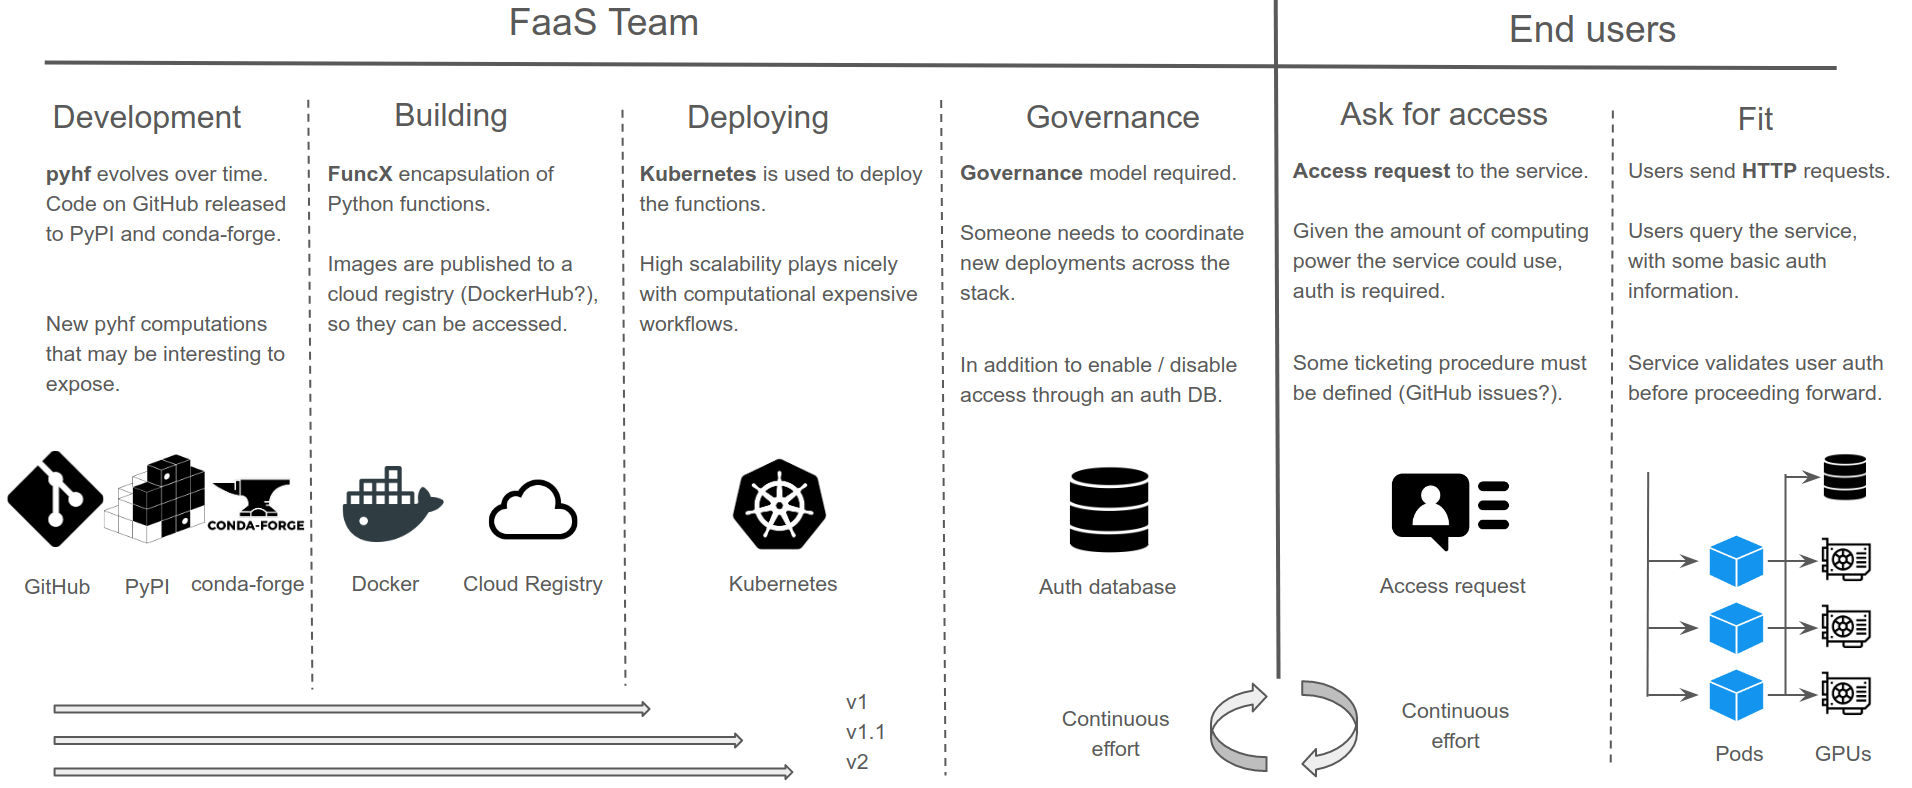
\includegraphics[width=\textwidth]{infrastructure_perspective.png}
    \caption{Example infrastructure design from the developer and user perspectives for a \pyhf{} and \funcX{} based fitting FaaS system for physics analysis.~\cite{portable_inference_workshop}}
    \label{fig:infrastructure_perspective}
\end{figure}
